\documentclass[10pt,twocolumn,a4paper]{ctexart}
\usepackage{amsmath,amssymb,amsthm}
\usepackage{booktabs,multirow,array}
\usepackage{graphicx}
\usepackage[table]{xcolor}
\usepackage{tikz}
\usetikzlibrary{arrows.meta,positioning,fit,calc,backgrounds}
\usepackage[hidelinks]{hyperref}
\usepackage{balance}
\usepackage{url}
\usepackage{cite}
\usepackage[a4paper,top=1.6cm,bottom=1.5cm,left=1.65cm,right=1.65cm,columnsep=0.62cm]{geometry}
\setCJKmainfont[AutoFakeBold=2,AutoFakeSlant=.2]{SimSun}
\setCJKsansfont[AutoFakeBold=2]{Microsoft YaHei}
\setmainfont{Times New Roman}
\graphicspath{{figures/}}
\definecolor{rulec}{HTML}{5A5A5A}
\definecolor{rfc}{HTML}{2F6DA8}
\definecolor{floorc}{HTML}{0E7C6B}
\definecolor{dangerc}{HTML}{C0392B}
\definecolor{evc}{HTML}{8A6D3B}
\colorlet{neutc}{black!60}
\newcommand{\CtoA}{C$\rightarrow$A}
\newcommand{\CtoB}{C$\rightarrow$B}
\newcommand{\BtoA}{B$\rightarrow$A}
\newcommand{\AtoB}{A$\rightarrow$B}
\newcommand{\Lsafe}{L_{\mathrm{safe}}}
\newtheorem{proposition}{命题}
\renewcommand{\figurename}{图}
\renewcommand{\tablename}{表}
\title{面向堤防渗流稳定透明评价的安全约束方法：\newline 学习等级的序数物理下限与巡检证据状态控制}
\author{作者信息待补充\thanks{内部工作稿，修订日期：2026 年 10 月。作者、单位、基金和目标期刊信息待内部确认。}}
\date{}
\begin{document}
\maketitle
\begin{abstract}
堤防渗流评价正在同时使用物理规则链、数据驱动分类器和无人机巡检，但单一安全等级无法说明学习模型是否降低了已识别的物理风险，也无法说明巡检候选是否经过确认。本文将透明评价表述为一条可审计的决策链，引入显式证据状态，并检验一种安全约束：序数物理下限允许随机森林提高物理规则链给出的等级，但不允许其降低该等级。在 875 条受控合成场景上，采用分组五折样本外预测，阈值随机森林将准确率由 0.845 提高至 0.873，但其漏判的关键等级样本全部变为直接的 C$\rightarrow$A 降级。在 10,000 组阈值中，没有任何组合消除这些错误，因为学习特征在所有严重度的穿结构场景中完全相同。序数下限混合模型达到 0.926 的准确率和 0.912 的宏平均 F1，修正规则链 136 个错误中的 71 个且未引入新错误，并消除了所有关键等级低估。在 5 个附加生成种子上，其准确率为 $0.921\pm0.004$，关键等级召回率为 $0.998\pm0.004$。该机制具有明确的代数性质：混合模型只有在两个组成部分同时低估时才会低估，并继承两个组成部分的过估计。在现场资料中，9 个经复核的红外管涌候选均未被确认，候选精度的单侧 95\% 精确上界为 0.28；未经复核的检测结果不能作为已确认事件进入安全等级。上述结论限于同一合成生成器，真实场地精度仍需独立现场标签验证。
\end{abstract}
\noindent\textbf{关键词：}堤防渗流；管涌；透明评价；物理约束机器学习；随机森林；序数安全等级；证据溯源；无人机红外巡检

\section{引言}
堤坝和堤防的内部侵蚀与漫顶是历史失事的重要机制。大型土石坝失事统计表明，堤身、地基或接触带管涌占据较高比例，砂性地基上的反向侵蚀管涌仍是堤防安全控制中的关键机制~\cite{Foster2000,vanBeek2015}。工程管理者并不直接依据这些机制行动，而是依据一个安全等级进行巡查、复核和处置。该等级需要把土层结构、水力边界、局部渗透坡降、边坡稳定性以及可见或热异常等信息压缩成一个序数结果。

两个趋势使这种压缩更难审计。第一，堤防数字孪生逐步把三维地质、渗流数值场和空基巡检放入同一场景~\cite{Fuller2020,Hou}，但输入可能存在时间过期、空间错配或仅为候选状态的问题。第二，数据驱动分类器开始与规则指标并行使用~\cite{Xu,Chen}。分类器可以提高总体准确率，却可能改变错误方向；在序数安全等级中，把关键等级 C 判为安全等级 A 与把安全等级 A 判为 B 的风险含义不同。

已有研究分别讨论了管涌可靠度更新~\cite{Schweckendiek,Roscoe,Baecher2003}、证据理论融合~\cite{Shafer1976,Chen}、理论引导机器学习~\cite{Karpatne2017,Rudin2019}以及代价敏感学习和拒识机制~\cite{Elkan2001,Chow1970,Geifman2017}。然而，仍缺少一个明确的决策层规则来回答：学习等级如何与物理规则等级组合，才能避免产生假安全降级；什么结构属性决定组合是否有效；未确认的巡检证据如何进入评价而不改变结论。

本文回答三个问题：Q1，在控制数据泄漏的验证下，随机森林是否优于物理规则链，其错误方向如何变化？Q2，单调的物理下限能否消除假安全错误，同时保留学习模型的有效修正，其保证条件是什么？Q3，如何表示巡检候选和不完整工程资料，使其不能在未确认的情况下静默改变安全等级？本文贡献包括：
\begin{itemize}
\item 建立证据状态、可采纳性和版本化运行协议，区分缺失、不适用、候选、已复核和可采纳证据，并记录进入等级结果的每个值的来源；
\item 建立分组样本外验证和错误方向指标，证明学习层的假安全错误来自特征盲区，而非单纯阈值选择；
\item 提出序数物理下限，给出其错误集合命题，并在原始批次、5 个附加种子、下限范围消融和复核预算实验中验证；
\item 将无人机红外候选和工程案例作为证据状态与溯源测试，而不是误称为现场预测精度验证。
\end{itemize}
本文的定量结果均来自同一合成生成器和其附加种子。因此，结果证明的是决策协议的行为及其失效条件，而不是现场范围内的预测准确率。

\section{相关研究}
\subsection{渗流安全的物理与数值证据}
隐式地质建模可利用钻孔与剖面资料插值地层界面，插值方法和条件数据共同决定最终几何形态~\cite{Wellmann2018,GemPy}。非稳定渗流通常采用 Richards 类方程描述，并结合 van Genuchten 关系表达非饱和土特性~\cite{Richards,Celia1990,vanGenuchten1980}；管涌模型则利用出口坡降描述侵蚀演化~\cite{vanBeek2015}。可靠度与贝叶斯更新可以传播参数变异并纳入历史观测~\cite{Schweckendiek,Roscoe,Baecher2003,Xu}，但这些方法没有规定特定材料区、场景和版本产生的响应何时可以作为运行等级的可采纳输入。

\subsection{数字孪生与溯源}
数字孪生研究通常描述感知、模型更新、模拟和决策支持之间的循环~\cite{Fuller2020}，建筑信息模型也被用于结合堤防机理算法开展全寿命管理~\cite{Hou}。PROV-DM 等溯源标准描述实体、活动和代理之间的派生关系~\cite{PROVDM}。但虚实同步本身不能决定一条过期、未登记或仅为候选的观测是否可以约束安全决策。本文把孪生场景作为上下文，并单独定义证据可采纳性。

\subsection{学习型安全分类器与物理引导}
已有渗流可靠度研究使用代理分类器，也有研究将深度学习与 Dempster--Shafer 融合用于坝体渗流评价~\cite{Xu,Chen}。树模型可以处理异质指标之间的交互，并支持特征层面的审计~\cite{Quinlan,Breiman,Hastie2009,LundbergLee}。理论引导数据科学和可解释模型研究强调在高风险场景中引入科学约束~\cite{Karpatne2017,Rudin2019}。以往约束多作用于输入、损失或模型结构，较少在决策层直接约束错误方向。

\subsection{巡检候选与选择性决策}
无人机摄影测量和热红外可覆盖较长堤段，但需要空间配准、辐射校准和飞行元数据支撑推断~\cite{Colomina2014}。图像分割、目标检测和热成像深度学习可定位渗漏样异常，但水陆边界、植被、阴影和湿地面可能产生相似热对比~\cite{Ronneberger2015,Redmon2016,Kumar2025}。选择性分类和拒识机制把低置信度样本送入人工复核~\cite{Chow1970,Geifman2017}。在堤防应用中，拒识意味着生成工程师复核任务，因此需要测量复核率及其后续等级影响。

\section{透明评价方法}
图~\ref{fig:framework}给出了决策链。证据首先经过可采纳性门控，物理规则链和学习层分别给出等级，序数物理下限进行组合，低置信度记录可进入复核。每个输出同时携带触发门控、证据状态以及模型和数据版本。

\begin{figure*}[t]
\centering
\begin{tikzpicture}[font=\footnotesize,>={Stealth[length=4pt]},box/.style={draw=#1,fill=#1!7,rounded corners=2pt,align=center,inner sep=3pt,line width=.55pt},lab/.style={font=\scriptsize\itshape,text=black!70,align=center},arr/.style={->,line width=.6pt,draw=black!65}]
\node[box=evc,text width=2.55cm] (geo) at (0,1.62) {地质与材料\\[-1pt]{\scriptsize 地层、土性参数}};
\node[box=evc,text width=2.55cm] (see) at (0,.54) {渗流场\\[-1pt]{\scriptsize 坡降、$i/i_{cr}$、FoS}};
\node[box=evc,text width=2.55cm] (his) at (0,-.54) {历史与记录\\[-1pt]{\scriptsize 事件、代码版本}};
\node[box=evc,text width=2.55cm] (uav) at (0,-1.62) {无人机红外巡检\\[-1pt]{\scriptsize 候选框}};
\node[lab] at (0,2.38) {证据通道};
\node[box=neutc,text width=2.45cm,minimum height=3.75cm] (adm) at (3.35,0) {\textbf{可采纳性门控}\\$a_j=1$ 当且仅当支持范围、\\有效时间和版本相容\\证据状态：可采纳、缺失、\\不适用、候选、已复核};
\foreach \n in {geo,see,his,uav} \draw[arr] (\n.east)--(\n.east-|adm.west);
\node[box=rulec,text width=3.15cm] (rule) at (7.0,.95) {\textbf{物理规则链}\\29 个指标 $\rightarrow R_m\rightarrow S$\\观测上限 $\rightarrow$ 硬门控};
\node[box=rfc,text width=3.15cm] (rf) at (7.0,-.95) {\textbf{学习层（RF）}\\14 个特征 $\rightarrow(p_A,p_B,p_C)$\\阈值 $(\tau_C,\tau_B)$};
\draw[arr] (adm.east|-rule.west)--node[above,font=\scriptsize]{可采纳} (rule.west);
\draw[arr] (adm.east|-rf.west)--node[below,font=\scriptsize]{可采纳} (rf.west);
\node[box=floorc,text width=2.5cm,line width=.9pt] (floor) at (10.6,0) {\textbf{序数物理下限}\\$\hat y=\max(\hat y_{RF},y_{rule})$};
\draw[arr] (rule.east)--(floor.north west);\draw[arr] (rf.east)--(floor.south west);
\node[font=\scriptsize,text=floorc,align=center] at (10.6,-1.0) {可提高风险等级，\\不能降低物理等级};
\node[box=neutc,text width=2.0cm] (rev) at (13.45,-.75) {\textbf{复核门}\\$\max_c p_c<u$\\$\rightarrow$ 工程师};
\node[box=neutc,text width=2.0cm] (out) at (13.45,.95) {\textbf{等级与溯源}\\门控、状态、版本};
\draw[arr] (floor.east)--(rev.west);\draw[arr] (rev.north)--(out.south);
\draw[arr,dashed,draw=dangerc] (uav.south)--++(0,-.42)-|node[pos=.25,below,font=\scriptsize,text=dangerc]{候选 $\rightarrow$ 复核任务，不能直接作为确认事件}(rev.south);
\end{tikzpicture}
\caption{堤防渗流透明评价决策链。规则链和学习层分别输出等级，序数物理下限对二者进行安全约束；巡检候选只有在时间、位置和人工状态闭合后，才能形成可采纳事件。FoS 表示安全系数。}
\label{fig:framework}
\end{figure*}

\subsection{评价单元、证据状态与可采纳性}
评价记录由 $(s,w,t,v)$ 索引，分别表示堤段、水力场景、观测或模拟时间以及证据和规则版本。每个指标保留原始值、单位、转换分数、来源位置、值类型、适用性、可用性、时间窗口、空间支持和转换规则。适用性与可用性分开处理：只有在确认相应设施或失效模式不存在时，指标才可标记为“不适用”；应当评价但尚未取得证据时标记为“缺失”。巡检证据进一步区分“候选”“已复核”和“可采纳”。只有时间、位置和状态闭合的确认事件才能施加确定性的管涌约束。

依据 PROV-DM，证据表可表示为有向溯源图~\cite{PROVDM}。对评价单元 $(s,w,t,v)$，指标 $x_j$ 的可采纳性定义为
\begin{equation}
a_j(s,w,t,v)=\mathbf{1}\{\mathcal{S}_j\cap\mathcal{S}_s\neq\varnothing\}\mathbf{1}\{t\in\mathcal{T}_j\}\mathbf{1}\{v_j\preceq v\}.
\label{eq:admissibility}
\end{equation}
当 $a_j=0$ 时，原始值保留用于追溯，但不得进入普通评分。空间错配的巡检框或过期模拟结果因此表现为溯源失败，而不是数值零值。

\subsection{物理规则链}
规则链包含 29 个二级指标和 5 个失效模式：漫顶、渗流、边坡失稳、冲刷和穿结构效应。令 $R_m\in[0,1]$ 为管理屏障修正后的模式响应，$\pi_m$ 为归一化权重，$\alpha$ 为短板系数，则
\begin{align}
\rho&=\alpha\max_mR_m+(1-\alpha)\sum_m\pi_mR_m,\\
S&=100(1-\rho),
\end{align}
其中 $\alpha=0.45$。$S\geq80$ 为 A 级，$40\leq S<80$ 为 B 级，$S<40$ 为 C 级。随后依次执行观测上限和物理硬门控。各阶段只能保持等级或将等级移向更高风险，不能将其移向更低风险。主导失效模式是内部响应最大的模式，不代表经过标定的失事概率。

\subsection{学习模型}
学习层使用 14 个物理和巡检特征：堤顶高程、地基/堤身/接触带坡降、上下游边坡安全系数、冲刷深度、巡检异常密度和证据等级、3 个除以 0.25 的坡降、下游安全系数倒数以及除以 1.0 m 参考值的冲刷深度。模型不使用目标模式、目标严重度、已给等级、综合分数、风险量或主导模式。14 个特征没有结构状态指标。

决策树和随机森林均为确定性的 NumPy CART 实现，使用 Gini 不纯度~\cite{Quinlan,Hastie2009}。决策树最大深度为 5，最小叶节点为 5；随机森林包含 120 棵自助采样树，最大深度为 7，最小叶节点为 3，每次分裂随机抽取 4 个特征~\cite{Breiman}。代价加权模型按 $w_C\in\{1.5,2,3,4,6\}$ 对 C 类进行加权抽样~\cite{Elkan2001}。所有超参数在附加种子生成前固定。概率向量是受控目标构造下的决策支持分数，不是现场失事概率。

\subsection{阈值策略、安全损失与 Pareto 比较}
阈值策略定义为
\begin{equation}
\hat y_{RF}=\begin{cases}C,&p_C\geq\tau_C,\\B,&p_C<\tau_C\text{ 且 }p_B\geq\tau_B,\\A,&\text{其他情况}.
\end{cases}
\label{eq:threshold}
\end{equation}
评价指标包括准确率、宏平均 F1、平衡准确率、C 类召回率、C 类低估方向、A 类过估计和升级率。安全损失定义为
\begin{equation}
\Lsafe=2N(C\rightarrow A)+N(C\rightarrow B),
\label{eq:safeloss}
\end{equation}
直接两级降级的权重是一级降级的两倍。若不存在另一组阈值在宏平均 F1、平衡准确率和 C 类召回率上不低于当前策略、在 $\Lsafe$ 上不高于当前策略，并且至少一个目标严格更优，则当前策略为非支配策略。升级率作为运行资源指标单独报告。按此定义，纯 RF 前沿在两种网格上都退化为一个目标向量，因为所有阈值均有 $\Lsafe\geq100$，阈值本身不提供质量–安全权衡。代表性工作点 $(0.35,0.20)$ 在 0.05 网格上选取，条件是 A 类无过估计、C 类召回率至少为 0.85，并在其中取得最高宏平均 F1。它是声明的运行点，不是工程最优点。另用 0.01 网格的 10,000 组阈值检验单纯调阈值能否消除 \CtoA{}。

\subsection{序数物理下限}
将 A、B、C 编码为 0、1、2。给定学习等级 $\hat y_{RF}$ 和规则链最终等级 $y_{rule}$，序数物理下限为
\begin{equation}
\hat y_H=\max(\hat y_{RF},y_{rule}).
\label{eq:veto}
\end{equation}
该策略不重新训练任何组成部分，同时保留证据溯源和触发门控。其错误行为遵循以下命题。
\begin{proposition}
对参考等级 $y$，有：(i) $\hat y_H<y$ 当且仅当 $\hat y_{RF}<y$ 且 $y_{rule}<y$；(ii) $\hat y_H>y$ 当且仅当 $\hat y_{RF}>y$ 或 $y_{rule}>y$；(iii) $\hat y_H=0$ 当且仅当两个组成部分都返回 0。因此，混合模型低估集合是两个组成部分低估集合的交集，过估集合是二者的并集，并且混合模型产生 \CtoA{} 的条件是规则链产生 \CtoA{}。
\end{proposition}
\begin{proof}
对整数 $a,b,y$，有 $\max(a,b)<y\Leftrightarrow a<y\wedge b<y$，$\max(a,b)>y\Leftrightarrow a>y\vee b>y$；对非负整数 $a,b$，$\max(a,b)=0\Leftrightarrow a=b=0$。
\end{proof}

方法按版本化决策协议执行：冻结 $(s,w,t,v)$，标记证据状态并排除不可采纳值，独立计算规则链和学习层，应用序数下限并记录学习等级被提高的级数；安全损失只在存在参考等级的离线评价中计算；低置信度或巡检候选生成复核任务后再发布等级。输出保留等级、触发门控、证据状态、溯源记录、模型版本和复核状态。阈值扫描确定学习层工作点，下限、复核预算和可采纳性规则共同决定部署条件。

\section{数据与验证协议}
\subsection{受控基准}
基准由冻结生成器产生，共包含 875 条记录：7 类目标模式（安全参考、漫顶、渗流、边坡、冲刷、穿结构和混合）$\times$5 个严重度$\times$25 条记录。参考等级遵循固定映射：安全和轻微对应 A（350 条），中等对应 B（175 条），严重和关键对应 C（350 条）。这是用于测试生成器内决策行为的封闭集合参考，不是现场安全标签。规则链最终等级依据交付的最终等级错误追踪重建，生成器回放与 5 个交付基准文件逐字节一致。

\subsection{划分与验证层级}
875 条记录包含 722 个不同的 14 维特征向量。相同向量被分配到同一折，所有学习结果采用分组五折样本外预测，以避免重复输入跨折泄漏~\cite{Kaufman2012,Roberts2017}。另有五外三内的分组嵌套验证在外层折内重新选择阈值。验证分为三层：原始 875 条记录用于检验冻结参考下的行为；5 个附加 875 条批次用于检验生成器实现变化；巡检与工程资料用于检验证据状态和溯源接口。后两类不用于声称外部预测准确率。

\subsection{统计分析}
与规则链的配对比较采用逐记录正确性上的精确双侧 McNemar 检验~\cite{McNemar1947,Dietterich1998}。混合模型相对规则链的批内不确定性采用按 722 个特征向量分组的配对百分位 Bootstrap，重采样 2,000 次~\cite{Efron1993}。5 个附加种子仅报告均值和样本标准差，不进行总体推断。对于 0/9 个确认现场候选，报告精确 Clopper--Pearson 上界~\cite{Clopper1934}。

\begin{table*}[t]
\caption{875 条受控记录上的分组五折样本外比较。C$\rightarrow$A 和 C$\rightarrow$B 表示 C 类低估，A$\uparrow$ 表示 A 类过估，Esc. 为输出 C 等级的比例。}
\label{tab:main}
\centering\footnotesize
\setlength{\tabcolsep}{3.2pt}
\begin{tabular}{@{}llccccrrrrc@{}}
\toprule
类别&方法&准确率&宏F1&平衡准确率&C召回&C$\rightarrow$A&C$\rightarrow$B&$\Lsafe$&A$\uparrow$&升级率\\
\midrule
物理&规则链&.845&.827&.847&.837&0&57&57&54&.335\\
\midrule
\multirow{5}{*}{学习层}&决策树&.707&.646&.635&.631&129&0&258&0&.253\\
&RF，多数投票&.829&.784&.763&.854&51&0&102&0&.342\\
&RF，阈值 $(.35,.20)$&.873&.858&.836&.857&50&0&100&0&.343\\
&RF，0.01 网格最优&.887&.890&.882&.857&50&0&100&24&.361\\
&RF，C 权重 6&.707&.701&.683&1.000&0&0&0&179&.683\\
\midrule
\multirow{3}{*}{下限策略}&RF+C-only&.930&.903&.884&1.000&0&0&0&0&.400\\
&\cellcolor{floorc!10}RF+序数下限&\cellcolor{floorc!10}.926&\cellcolor{floorc!10}.912&\cellcolor{floorc!10}.928&\cellcolor{floorc!10}1.000&\cellcolor{floorc!10}0&\cellcolor{floorc!10}0&\cellcolor{floorc!10}0&\cellcolor{floorc!10}54&\cellcolor{floorc!10}.400\\
&RF+下限+复核 $u=.60$&.911&.896&.914&.966&0&12&12&54&.386\\
\bottomrule
\end{tabular}
\end{table*}

\begin{figure*}[t]
\centering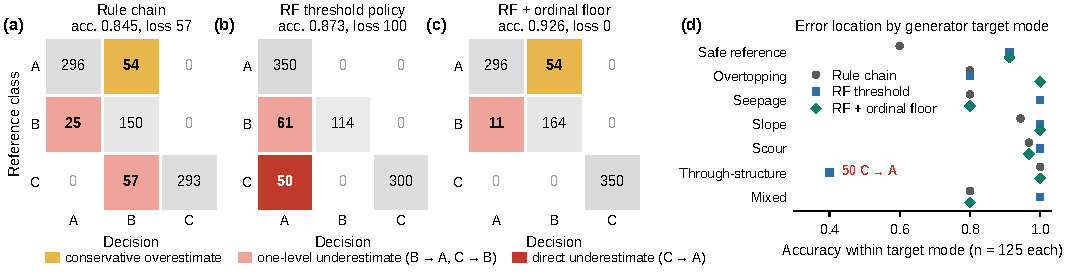
\includegraphics[width=\textwidth]{fig_error_structure.pdf}
\caption{875 条受控记录上的错误结构。(a)--(c) 分别为规则链、RF 阈值策略和序数下限混合策略的混淆矩阵；(d) 为各目标模式内的准确率。RF 的所有 \CtoA{} 错误均出现在穿结构模式，该模式所有记录共享一个 14 维特征向量。}
\label{fig:errors}
\end{figure*}

\section{结果}
\subsection{规则链具有保守错误，硬门控决定主要表现}
规则链正确分类 739/875 条记录，准确率 0.845，宏 F1 0.827，平衡准确率 0.847。全部 136 个错误均为一级错误，其中包括 54 个 \AtoB{}、25 个 \BtoA{} 和 57 个 \CtoB{}，没有 \CtoA{} 或 A$\rightarrow$C。评分本身仅正确分类 450 条记录；观测上限没有改变等级，硬门控改变了 322 条记录。去除巡检指标后，150 个分数发生最多 1.39 分的变化，但没有等级变化。

\subsection{学习策略提高总体指标，但产生假安全降级}
浅层决策树在所有总体指标上都低于规则链。多数投票 RF 将 C 召回率从 0.837 提高到 0.854，但准确率和宏 F1 下降，其 51 个 C 类漏判全部为直接 \CtoA{}，安全损失由 57 增至 102。代表性阈值策略准确率为 0.873，宏 F1 为 0.858；与规则链的正确性差异不显著，精确 McNemar $p=0.11$。其 50 个 C 类漏判同样全部为 \CtoA{}，安全损失为 100。

在 10,000 组 0.01 网格阈值中，没有任何组合将 \CtoA{} 降至 50 以下。宏 F1 最优组合 $(0.19,0.06)$ 达到 0.890，但产生 24 个 A 类过估计。代价权重达到 6 时才消除 \CtoA{}，但准确率降至 0.707，并将 350 个 A 类样本中的 179 个升级。问题来自特征盲区而非阈值选择：所有 50 个 \CtoA{} 错误均出现在穿结构模式，其中 125 条记录从安全到关键共享完全相同的特征向量。任何仅依赖这些特征的函数都无法分离严重度。

\subsection{序数下限消除低估且不增加相对规则链的新错误}
混合模型准确率 0.926，宏 F1 0.912，平衡准确率 0.928，C 召回率 1.000，安全损失为 0。相对规则链，它修正 136 个错误中的 71 个且没有引入新错误，精确 McNemar $p<10^{-20}$。分组 Bootstrap 显示准确率提高 8.1 个百分点（95\% 区间 5.4--11.5），宏 F1 提高 8.5 个百分点（6.0--11.3），安全损失降低 57（-72-- -42）。

相对 RF 阈值策略，混合模型改变 154 个决策，修正 100 个 RF 错误并产生 54 个 \AtoB{} 升级，这些升级正是规则链的保守错误。C-only 下限准确率更高，为 0.930，但平衡准确率降至 0.884；在附加种子中，它曾产生直接 \CtoA{}，而完整序数下限将其限制为 \CtoB{}。去除两个巡检特征后，混合模型准确率降至 0.917，并出现 1 个 \CtoB{}，说明合成巡检特征对学习层有少量信号，但对规则链等级没有作用。

\begin{figure}[t]
\centering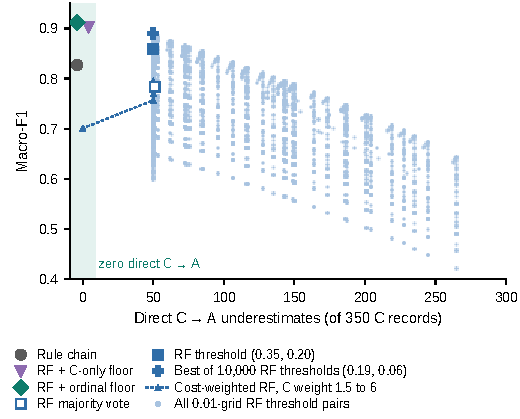
\includegraphics[width=\columnwidth]{fig_safety_tradeoff.pdf}
\caption{质量指标与直接 \CtoA{} 错误的关系。所有纯 RF 阈值至少产生 50 个 \CtoA{}；只有规则链、C 权重 6 的 RF 和两种下限策略达到零直接降级。}
\label{fig:tradeoff}
\end{figure}

\subsection{附加生成种子上的稳健性}
在 5 个附加批次中，序数下限相对规则链均未引入新错误，每个种子修正 61--68 个规则链错误，准确率、宏 F1 和平衡准确率分别提高 $7.4\pm0.3$、$7.7\pm0.4$ 和 $7.1\pm0.5$ 个百分点。RF 阈值策略相对规则链的准确率优势只有 5 个种子中的 1 个达到 $p<0.05$。在种子 20260932 中，两个组成部分共同漏判 3 个 C 类记录，完整序数下限输出 B，而 C-only 下限输出 A。多数投票 RF 的 C 召回率为 $0.837\pm0.013$，低于规则链的 $0.842\pm0.002$。

\begin{figure*}[t]
\centering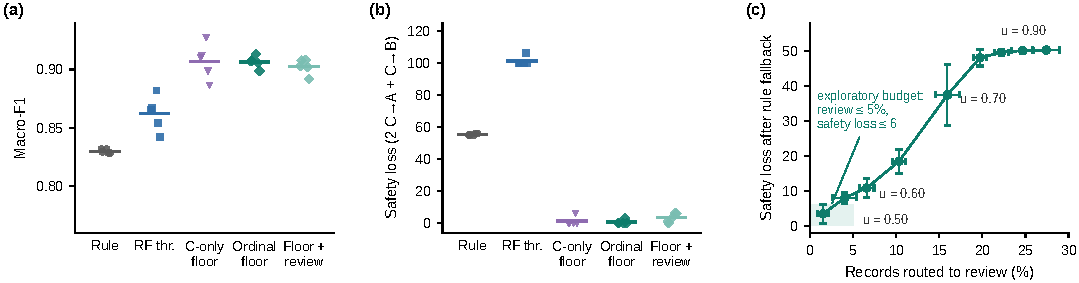
\includegraphics[width=\textwidth]{fig_multiseed_review.pdf}
\caption{5 个附加生成种子及复核预算结果。(a) 宏 F1；(b) 安全损失；(c) 复核阈值扫描。$u=.50$ 时平均复核率为 $1.5\pm0.7\%$，但离线规则链回退代理会损失部分学习层升级。}
\label{fig:seeds}
\end{figure*}

\subsection{复核预算}
在 $u=0.50$ 时，平均复核率为 $1.5\pm0.7\%$，C 召回率为 $0.990\pm0.008$，安全损失为 $3.4\pm2.8$；在 $u=0.60$ 时，复核率为 $6.6\pm0.9\%$，安全损失为 $10.8\pm2.8$。原始批次中，$u=.50$ 路由 7 条记录且不改变闭集指标，$u=.60$ 路由 62 条记录并产生 12 个 \CtoB{}。这些数字衡量的是“以规则链等级代替工程师复核”的代理成本，不是实际复核效果。复核阈值是在同一生成器族内事后选择的，外部评估前必须预先固定。

\subsection{巡检候选作为评价状态}
进入人工复核的 9 个现场候选均被判定为非管涌。检测置信度范围为 0.466--0.777，原因包括水陆边界热对比、植被与阴影、建筑边缘热惯性与阴影，以及湿地面或镜头边缘渐晕。0/9 确认事件对应候选精度单侧 95\% 精确上界 0.28。13 张人工管涌图像中的 14 个检测框置信度较高，但没有漏检记录，因此不能估计召回率或现场迁移能力。

\begin{figure}[t]
\centering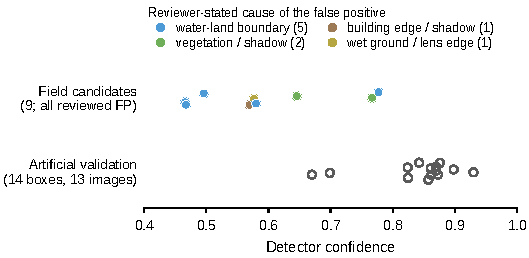
\includegraphics[width=\columnwidth]{fig_inspection_status.pdf}
\caption{9 个经复核现场候选和 14 个人工管涌图像检测框的置信度。候选框按复核原因着色；人工管涌图像不具有复核状态和漏检记录。}
\label{fig:inspection}
\end{figure}

候选可以生成复核任务，但在时间、位置和人工状态闭合前不能作为确认管涌事件进入等级；未检查图像应保留为未观测状态，而不是“无异常”。两个最高置信度现场候选（0.777 和 0.767）分别来自水陆边界和植被，说明仅依靠置信度阈值不能把它们与真实渗漏分开。

\subsection{工程案例溯源}
K45+500 交付案例给出 C 级、渗流主导、分数 24.35。该案例存在 15/29 指标缺失、指标表与结果文件之间 4 项冲突、评价模块版本差异以及历史管涌信息进入输入等问题。水位是代表性高水位场景而非实测 2017 年水位。因此，该案例证明接口能够暴露资料问题，但不能作为独立预测验证。

\section{讨论}
本文的安全收益来自组合规则，而不是学习器本身。森林模型只在总体指标上取得有限改善，并在各批次中将关键等级漏判变为直接降级；序数下限消除了这些降级，同时保留了大部分有效修正。命题说明，方法在两个组成部分错误互补且学习层过估计较少时最有价值，并继承规则链的所有保守错误。

该方法位于理论引导学习与拒识策略之间。理论引导学习把物理知识放入输入、损失或模型结构~\cite{Karpatne2017}，序数下限则在决策层约束学习层影响方向。它比可靠度概率更新简单，但不替代可靠度方法。与拒识不同，序数下限本身不放弃决策；复核的价值取决于真实工程师信息，而当前实验只能用规则等级作为离线代理。

两个因素限制收益大小。首先，规则链硬门控与生成器严重度构造存在对齐，混合模型相对纯学习器的部分优势可能由基准结构带来。其次，森林特征缺少结构状态指标，补充这些特征后，学习器盲区可能缩小。二者都不削弱下限的保护作用，但说明方法不能替代独立现场验证。

本文结论受四方面边界约束：全部定量比较来自同一合成生成器；序数保证以规则链为条件，规则链若整体漏判关键状态，错误会传递到混合模型；复核预算使用规则回退代理，不是工程师复核实测；现场资料仅有 9 个经复核候选和 1 个非盲工程案例，不能给出检测或预测精度。下一步需要带有独立标签、时间记录和空间配准的现场数据，补充结构状态特征，并记录真实复核决策。

\section{结论}
本文提出了一种序数物理下限，使学习层可以提高但不能降低物理规则链给出的堤防渗流风险等级。在 6 个受控批次中，该方法相对规则链没有增加新错误，并消除了直接的关键到安全降级。其收益来自错误集合的交集性质：只有两个组成部分同时低估时才会低估，因此它依赖错误互补性，并且其防止直接降级的能力受规则链本身限制。将巡检结果保留为待复核候选，将工程交付资料作为溯源对象，可以防止未确认或不一致证据直接进入等级。真实场地标签是检验这种互补性是否能够迁移到合成生成器之外的下一步条件。

\section*{数据与代码可用性}
脱敏仓库包含受控基准及其生成器、附加种子、分析脚本、巡检审计表、本文及逐记录预测结果。论文修订所用统计和图件可由 \url{experiments/analysis/paper_revision/paper_statistics.py} 和 \url{make_paper_figures.py} 重新生成。原始现场图像在可行范围内移除了元数据，本文不报告位置。

\section*{致谢}
感谢项目组提供受控评价资料、工程案例材料和无人机巡检记录。作者和基金信息将在内部评审后补充。

\balance
\bibliographystyle{IEEEtran}
\bibliography{references}
\end{document}
